\hypertarget{_line_8h}{}\section{Coursework 2 -\/ starter/\+Coursework 2 -\/ starter/include/\+Line.h File Reference}
\label{_line_8h}\index{Coursework 2 -\/ starter/\+Coursework 2 -\/ starter/include/\+Line.\+h@{Coursework 2 -\/ starter/\+Coursework 2 -\/ starter/include/\+Line.\+h}}
{\ttfamily \#include $<$Box2\+D/\+Box2\+D.\+h$>$}\newline
{\ttfamily \#include $<$S\+F\+M\+L/\+Graphics.\+hpp$>$}\newline
{\ttfamily \#include $<$iostream$>$}\newline
{\ttfamily \#include \char`\"{}..\textbackslash{}include\textbackslash{}\+Level\+Loader.\+h\char`\"{}}\newline
Include dependency graph for Line.\+h\+:\nopagebreak
\begin{figure}[H]
\begin{center}
\leavevmode
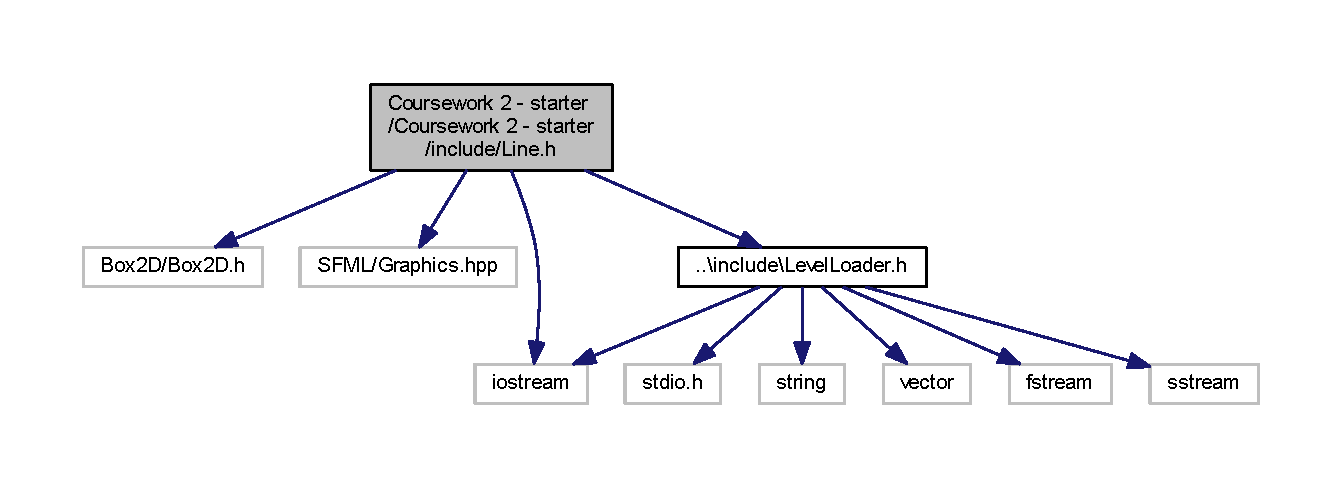
\includegraphics[width=350pt]{_line_8h__incl}
\end{center}
\end{figure}
This graph shows which files directly or indirectly include this file\+:\nopagebreak
\begin{figure}[H]
\begin{center}
\leavevmode
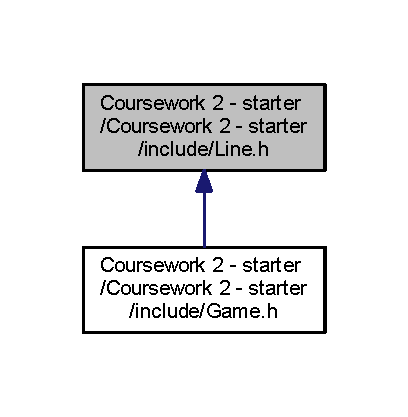
\includegraphics[width=196pt]{_line_8h__dep__incl}
\end{center}
\end{figure}


\subsection{Detailed Description}
This class draws and sets the line in the world.

This line is specifically used for acting as the ground which the player will drive around on with the bike. This class takes x amount of floats and sets them as vertices, it also creates a box2d chain object and draws an sfml line .the positions are loaded in from file to make it kind of easier to construct the level. the file reads two vertices and sets them as the line and draws them in random colour to give it a funky space look. 